\documentclass[../notes.tex]{subfiles}

\begin{document}

\section{Motion}

\subsection{Basic Concept of Motion}

\texttt{Distance} is a measurement of how far an object have traveled. 
Distance is a scaler.
The vector counterpart of distance, \texttt{displacement} ($s$) measures the distance from the start to the end of a motion.
It also includes the measurement of direction.
The SI Unit of displacement is \texttt{meters}.
If a object travels in a circle, the distance is the circumference of the circle, but the displacement \textit{would be zero}.

\texttt{Speed} denotes the rate of change of distance.
Speed is a vector.
\texttt{Velocity} measures both rate of change of displacement and change in direction.
A change in \textit{velocity} might not be a change in \texttt{speed}.

\texttt{Acceleration} is the change in velocity.
Acceleration is a vector.
There is no scaler equivalent of acceleration.
Acceleration also measures the change it direction.
Thus, in circular motion, an object is \textit{always} accelerating.

\subsubsection{Average Versus Instantaneous}
We commonly measure rate of change with respect to time.
For example, to find the velocity of a bike, we measure the displacement over a period of 5 seconds.
This is the average velocity.

Average velocity accounts for all the changes in velocity during the time period of measurement.
Instantaneous velocity is the velocity of the bike at the exact time.
This instantaneous velocity may not be exactly the same as the average velocity.

\section{Graphing Motion}
Often times, motion of an object can be graphed. 
These graphs gives us a lot of information.

\subsection{Position Time Graph}
\begin{figure}[h]
\begin{center}
	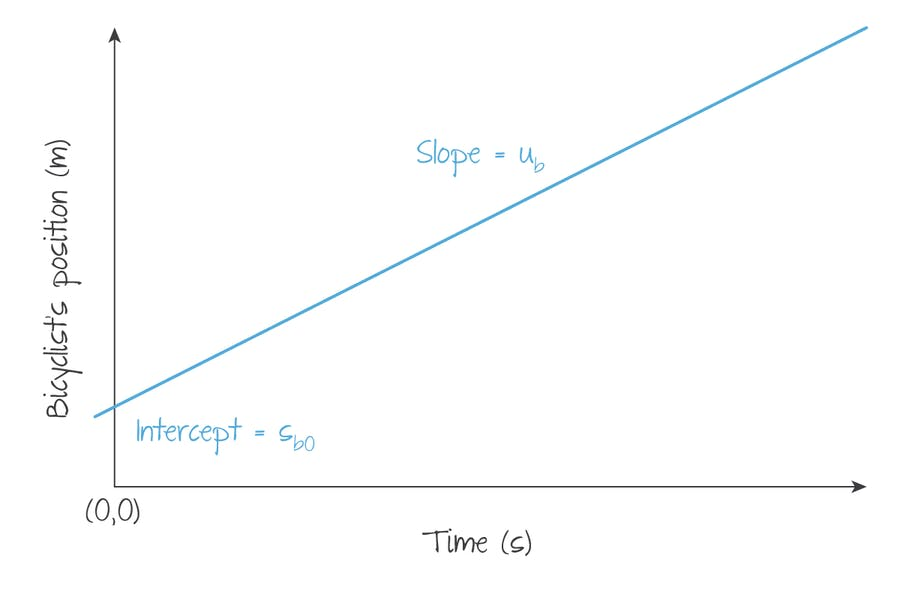
\includegraphics[width=\textwidth]{./figures/position-time.jpg}
	\caption{A position time graph of a bike over time}
\end{center}
\end{figure}

The change in Y values is the displacement.
The change in X value is the change in time.
The gradient of the line is the velocity.

\begin{figure}[h]
\begin{center}
	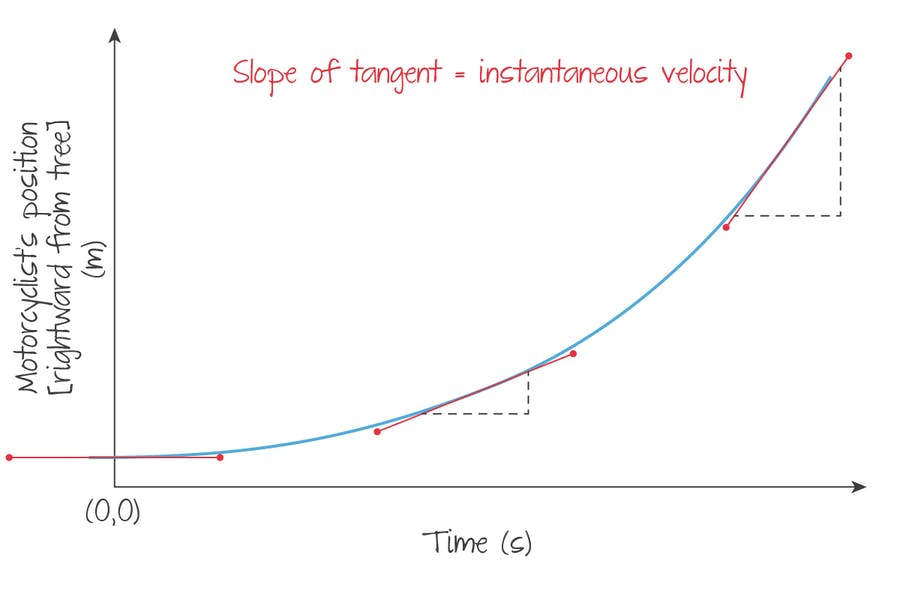
\includegraphics[width=\textwidth]{./figures/position-time-curve.jpg}
	\caption{A curved position time graph}
\end{center}
\end{figure}

Note, if the curve is non-linear, the average velocity would be the average slope.
The instantaneous velocity is the slope of the tangent line.

\subsection{Velocity Time graph}
\begin{figure}[h]
\begin{center}
	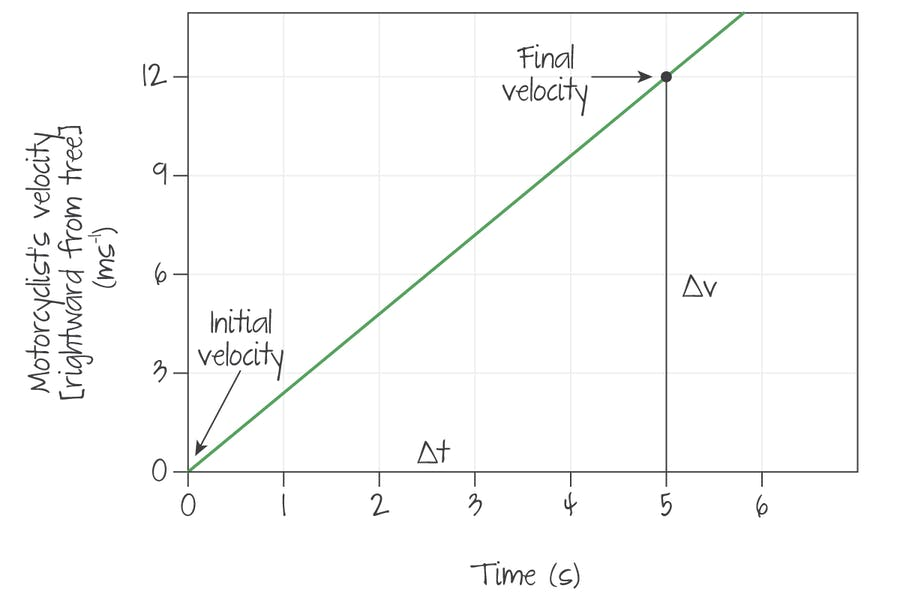
\includegraphics[width=\textwidth]{./figures/velocity-time.jpg}
\end{center}
\end{figure}

The Y intercept of the graph is the initial velocity.
The change in Y is the change in velocity.
The change in X is the change in time.
The gradient of the graph is the acceleration (use tangent line if we need the instantaneous acceleration).
The area under the curve is the displacement.

\subsection{Acceleration Time graph}
\begin{figure}[h]
\begin{center}
	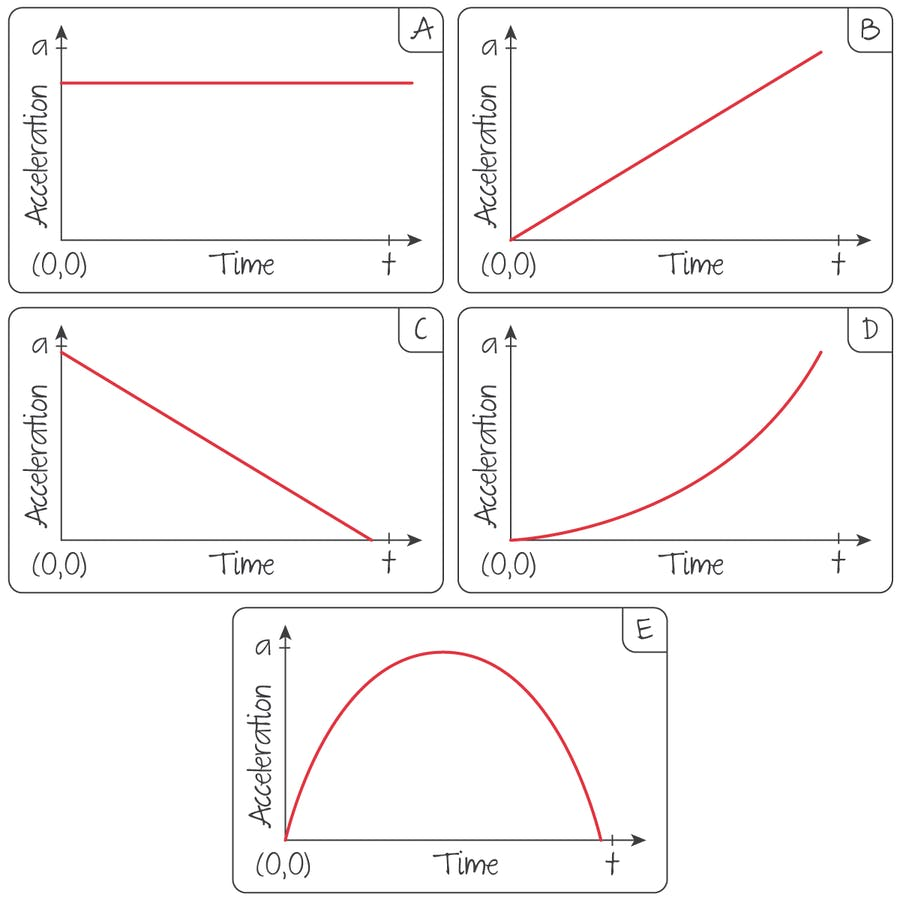
\includegraphics[width=\textwidth]{./figures/acceleration-time.jpg}
	\caption{Acceleration Time graph}
\end{center}
\end{figure}

The area under the curve is the change in velocity.

\subsection{Free fall air resistance}
\begin{figure}[h]
\begin{center}
	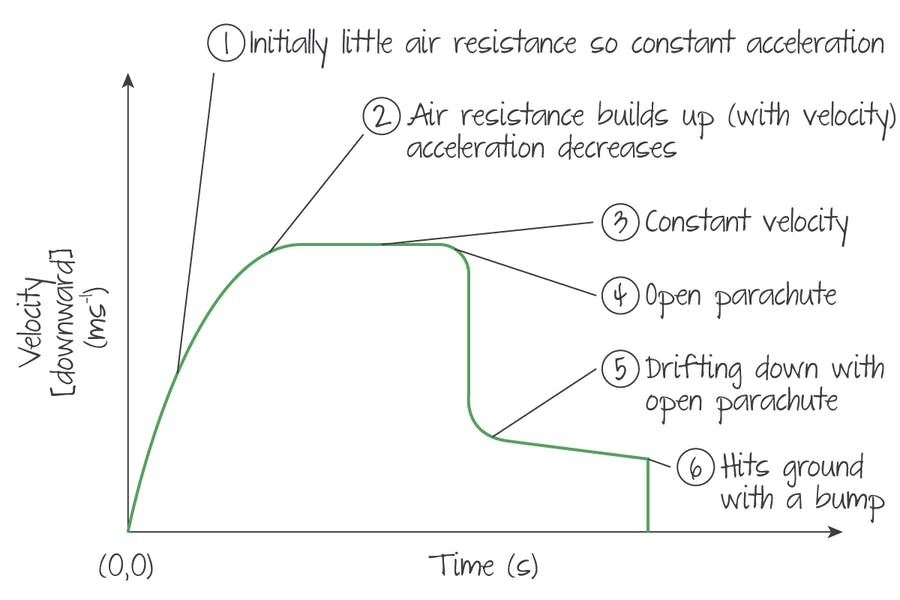
\includegraphics[width=\textwidth]{./figures/velocity-freefall.jpg}
	\caption{Velocity time graph of an object in free fall}
\end{center}
\end{figure}

\section{SUVAT}
The SUVAT equations describe the relationship acceleration, displacement, velocity, and time.

\begin{align}
	v = u + at \\
	s = ut + \frac{1}{2}at^2 \\
	v^2 = u^2 + 2as \\
	s = (\frac{v+u}{2})t
\end{align} 

$v$ final velocity, $u$ is initial velocity.
$t$ is time.
$a$ is acceleration.

\section{Projectile Motion}
In a projectile motion, a object is accelerated in a certain direction.
During flight, no additional force acts on said object.
Projectile motion ends when the object impact the ground.

When analyzing projectile motion, split the variables into horizontal and vertical components.
After the initial force, the horizontal acceleration is zero (horizontal velocity maintains constant), while the vertical acceleration remains constant ($g$, acceleration due to gravity).
To find the net force/acceleration/velocity, we can use Pythagorean Theorem to combine the $x$ and $y$ components.

\begin{align*}
	V_{net} = \sqrt{{V_{vertical}}^2 + {V_{horizontal}}^2}
\end{align*} 

\section{Forces}

\subsection{Newton's Laws of Motion}
\begin{enumerate}
	\item An object continues to remain stationary or to move at a constant velocity unless an external force acts on it.
	\item $F=ma$,  $f = \frac{\Delta mv}{t}$, impulse is equal to change in momentum.
	\item Every action has an equal and opposite reaction.
\end{enumerate}

\subsection{Free-Body Diagram}
Free body diagrams are often used to show the forces acting on an object.
Forces are drawn as arrows, with the direction of the arrow representing the direction of the force.
And the length of the arrow representing magnitude.
All forces need to have clear labels.

When drawing a free-body diagram, it is easier to represent the mass as a dot.
All arrows start from the dot.

Note, if an object falls a long period of time, it may hit terminal velocity.
This is when air resistance increases a velocity increases, and eventually counteracts the force due to gravity.

\subsection{Translational Equilibrium}
Net force is the combination of all the forces acting on a body.
Adding forces as vectors requires taking in account of direction.
An object will accelerate according to the net force.
If the net force of an object is zero, then the object is in translational equilibrium.
This means the object is moving at constant velocity, or stationary.

\section{Friction}
Solid friction is a type of friction that occurs where two surfaces are in contact.
There is two types of solid friction, static friction and dynamic friction.

\subsection{Static Friction}
Static friction occurs when there is no movement between two objects.
Static friction increases with the force acting on an object until hitting a certain point.
After reaching the point, the object begins to accelerate, and friction transfers to dynamic friction.

Static friction can be represented by:
\begin{equation}
	F_t \le \mu_s R
\end{equation}

\subsection{Dynamic Friction}
Dynamic friction happens when an object is moving.
Dynamic friction is modeled by this equation:
\begin{equation}
	F_t = {\mu}_d R
\end{equation}
Where $F_t$ is the force due to friction. 
$\mu$ is the coefficient of friction.
$R$ is the normal force acting on the object.

\section{Work, Energy, and Power}
Energy is stored in many forms.
Below is a list of some common ways of storing energy.
\begin{itemize}
	\item Kinetic
	\item Gravitational Potential
	\item Electric/Magnetic
	\item Chemical
	\item Nuclear
	\item Elastic
	\item Thermal
	\item Mass
	\item Vibration
	\item Light
\end{itemize}

Energy is often transformed into many different forms.
One way to describe energy is through work.

\subsection{Work}
Work ($W$), has the SI Unit of Joules ($J$).
The definition of work is the amount of energy required to move a mass of $1 kg$ over a distance of $1m$.
The equation for work is:
 \begin{equation}
	W = F \cdot s
\end{equation}
Where $s$ is displacement, and $F$ is force. 

Note, if the force is exerted at an angle to the direction of displacement, we have to use trig ratios to find the component of the force that is parallel to the direction of displacement.
Often times, work is multiplied by $\cos\theta$ (where $\theta$ is the angle between the force and the direction of motion) in order to account the difference in angles.

Sometimes, there is a resistive force done against the direction of travel.
In this case, there would be work done by the force and work done by the resistive force.

\subsection{Force Distance Graph}
In a force distance graph, area under the curve is the work done.

\subsection{Power}
Power ($P$) is defined as the rate of doing work.
The SI Unit of power is watts.
\begin{equation}
	P = \frac{W}{t}
\end{equation}
In which $t$ represents time.

\subsection{Kinetic Energy}
Kinetic Energy (KE) is defined as the energy objects have due to its motion.
The SI Unit of kinetic energy is Joules.
\begin{equation}
	KE = \frac{1}{2}mv^2
\end{equation}

\subsection{Gravitational Potential Energy}
Gravitational Energy (GPE) is defined as the energy an object gains due to its height.
\begin{equation}
	GPE = mgh
\end{equation}
In which, $m$ is mass, $g$ is the acceleration due to gravity, and $h$ is the height from a reference point. 

$g$ is a constant.
IB defines the acceleration due to gravitational on Earth's surface as $9.8 m\cdot s^{-2}$.

\subsection{Conservation of Energy}
In a close system, energy is always conserved.
For example, when dropping an object from a height, gravitational energy converts of kinetic energy.
You can write this in an equation:
\begin{equation}
	\frac{1}{2}mv^2 = mgh 
\end{equation}

Sometimes, there is some energy lost in the transition.
For example, kinetic energy may be lost to heat (thermal energy).

\subsection{Elastic Potential Energy}
The force due to elasticity can be modeled by Hooke's law.
\begin{equation}
	F = kx
\end{equation}
Where $x$ is the displacement from the spring's central position and $k$ is the spring constant.
The central point is also where the spring is at equilibrium, where the net force is zero.

\subsection{Efficiency}
The efficiency of a system is how much energy was useful.
\begin{equation}
	\textrm{efficiency} = \frac{ \textrm{useful work out} }{ \textrm{total energy in} }
\end{equation}

\section{Momentum}
Momentum ($p$) is the product of the mass of an object and its velocity.
\begin{equation}
	p = mv
\end{equation}
Where $p$ is momentum, $m$ is mass, and $v$ is velocity.
Momentum is a vector.

\subsection{Impulse}
The change in momentum is equals to impulse.
Impulse is defined by force multiplied by time.
\begin{equation}
	pv = ft
\end{equation}

\subsection{Conservation of Momentum}
In a close system, momentum is always conserved.
This means the change in momentum of one object may contribute to the change in momentum of another object.

\subsection{Force-Time Graphs}
The area under a force-time graph is the impulse, or the change in momentum.

\subsection{Collisions}
There is three types of collisions: elastic, inelastic, and completely inelastic collision.

In an elastic collision, kinetic energy of the system is conserved.
In an inelastic collision, some kinetic energy is waste, converted into heat, sound, etc.
In a completely inelastic collision, the two objects stick together, kinetic energy is not conserved.

Note, in all collisions, momentum is conserved.

In an explosion, momentum is not conserved, as there is an external force acting on the object.

\subsection{Energy and Momentum}
Since the equation for kinetic energy and momentum are both based on mass and velocity, we can find a relationship between the kinetic energy and the momentum of an object.
This is a useful shortcut.
\begin{equation}
	KE = \frac{p^2}{2m}
\end{equation}

\end{document}
